\section{Experiment Results}
In this section, we examine the attack effectiveness and robustness of our approach under extensive settings. 


\begin{table}[tb]
    \centering
    \setlength{\tabcolsep}{1mm}
    \vspace{-2ex}
    \resizebox{1\columnwidth}{!}{
    \begin{tabular}{l|ccc|ccc}
    \toprule
        \multirow{2}{*}{Methods} &  \multicolumn{3}{@{}c}{{\bf GSM8K}} &  \multicolumn{3}{@{}c}{{\bf BBH}} \\
         & EM & Tokens & $1/\tau$ & EM & Tokens & $1/\tau$\\
        % \hline
         \cmidrule (r){1-1}\cmidrule (lr){2-4} \cmidrule (lr){5-7}
     Full-shot & 78.85 & 2,366 & - & 70.07 & 774 & -  \\
     \hline
     \hline
     \multicolumn{4}{@{}l}{{\bf \textit{1-shot constraint}}} \\ 
    1-shot & 77.10 & 422 & 6x & 69.60 & 284 & 3x \\
    Selective-Context & 53.98 & 452 & 5x & 54.27 & 276 & 3x \\
    GPT4 Generation & 71.87 & 496 & 5x & 27.13 & 260 & 3x \\
    {\cellcolor[rgb]{0.925,0.957,1}}\textbf{Ours} & {\cellcolor[rgb]{0.925,0.957,1}}\textbf{79.08} & {\cellcolor[rgb]{0.925,0.957,1}}446 & {\cellcolor[rgb]{0.925,0.957,1}}5x & {\cellcolor[rgb]{0.925,0.957,1}}\textbf{70.11} & {\cellcolor[rgb]{0.925,0.957,1}}288 & {\cellcolor[rgb]{0.925,0.957,1}}3x \\
     \hline
     \hline
     \multicolumn{4}{@{}l}{{\bf \textit{half-shot constraint}}} \\ 
    Sentence Selection & 72.33 & 230 & 10x & 39.56 & 175 & 4x\\
    Selective-Context & 52.99 & 218 & 11x & 54.02 & 155 & 5x \\
    GPT4 Generation & 68.61 & 223 & 11x & 27.09 & 161 & 5x \\
    {\cellcolor[rgb]{0.925,0.957,1}}\textbf{Ours} & {\cellcolor[rgb]{0.925,0.957,1}}\textbf{77.41} & {\cellcolor[rgb]{0.925,0.957,1}}171 & {\cellcolor[rgb]{0.925,0.957,1}}14x & {\cellcolor[rgb]{0.925,0.957,1}}\textbf{61.60} & {\cellcolor[rgb]{0.925,0.957,1}}171 & {\cellcolor[rgb]{0.925,0.957,1}}5x \\
     \hline
     \hline
     \multicolumn{4}{@{}l}{{\bf \textit{quarter-shot constraint}}} \\ 
    Sentence Selection & 66.67 & 195 & 12x & 46.00 & 109 & 7x \\
    Selective-Context & 44.20 & 157 & 15x & 47.37 & 108 & 7x \\
    GPT4 Generation & 56.33 & 188 & 20x & 26.81 & 101 & 8x \\
    {\cellcolor[rgb]{0.925,0.957,1}}\textbf{Ours} & {\cellcolor[rgb]{0.925,0.957,1}}\textbf{77.33} & {\cellcolor[rgb]{0.925,0.957,1}}117 & {\cellcolor[rgb]{0.925,0.957,1}}20x & {\cellcolor[rgb]{0.925,0.957,1}}\textbf{56.85} & {\cellcolor[rgb]{0.925,0.957,1}}110 & {\cellcolor[rgb]{0.925,0.957,1}}7x \\
     \hline
     \hline
    zero-shot & 48.75$^{\dag}$ & 11 & 215x & 32.32 & 16 & 48x \\
    Simple Prompt & 74.9 & 691 & 3x & - & - & - \\
    \bottomrule
    \end{tabular}
    }
    \caption{Performance of different methods under different target compression ratios on the GSM8K mathematical reasoning and Big-bench Hard (BBH) datasets. $^{\dag}$We also include the instruction of the prompt in zero-shot experiments for a vertical comparison.}
    \label{tab:main_results}
\end{table}



\begin{table}[t]
\footnotesize{
    \centering
    \begin{tabular}{lcccc}
        \toprule
        \multirow{2}{*}{Defense Method} & \multicolumn{4}{c}{Attacking Effectiveness} \\ 
         &  SSIM $\downarrow$ & PSNR $\downarrow$ & LPIPS $\uparrow$ & IA-Score $\downarrow$ \\
        \midrule
        Crop-and-Resize & 0.68 & 29.28 & 0.42 & 0.79 \\
        JPEG Comp. & 0.78  & 29.82 & 0.36 & 0.79 \\
        \midrule
        None & 0.79 & 30.05 & 0.33 & 0.81 \\
        \bottomrule
    \end{tabular}
    \caption{Quantitative results of our adversarial images against defense methods. Both Crop-and-Resize and JPEG Compression fail to defend our attack. ``None'' indicates no defense is applied, as the baseline for comparison.}
    % The term "None" in the defense method column indicates the use of the adversarial image generated by our method without applying any purification techniques.
\label{tab:defense}
}
\end{table}



\subsection{Experiment Settings}
\subsubsection{Implementation Details.} We conduct all our experiments in white box settings and examine the effectiveness of our attacks using SDEdit \cite{meng2021sdedit}. For the Variational Autoencoder (VAE) ~\cite{kingma2014autoencoding} in our AtkPDM$^{+}$, we utilize the VAE provided by StableDiffusion V1.5 ~\cite{rombach2022high}.
We run all of our experiments with 300 optimization steps, which is empirically determined, to balance attacking effectiveness and image protection quality with reasonable speed. Other loss parameters and running time are provided in the Appendix. The implementation is built on the Diffusers library. All the experiments are conducted with a single Nvidia Tesla V100 GPU.


\subsubsection{Victim Models and Datasets.}
We test our approach on PDMs with three open-source checkpoints on HuggingFace, specifically ``google/ddpm-ema-church-256'', ''google/ddpm-cat-256'' and ``google/ddpm-ema-celebahq-256''. For the results reported in Table~\ref{tab:attackPDM}, we run 30 images for each victim model. Additionally, for generalizability in practical scenarios, we synthesize the data with half randomly from the originally trained dataset and another half from randomly crawled with keywords from the Internet.

\subsubsection{Baseline Methods and Evaluation Metrics.}

To the best of our knowledge, previous methods have mainly focused on LDMs, and effective PDM attacks have not yet been developed, however, we still implement Projected Gradient Ascent (PGAscent) with their proposed semantic loss by~\cite{salman2023raisingcostmaliciousaipowered, liang2023adversarialexampledoesgood, liang2023mistimprovedadversarialexamples, xue2024effectiveprotectiondiffusionbased}. Notably, Diff-Protect~\cite{xue2024effectiveprotectiondiffusionbased} proposed to minimize the semantic loss is surprisingly better than maximizing the semantic loss, we also adopted this method in attacking PDMs and denote as Diff-Protect. To quantify the adversarial image visual quality, we adopted Structural Similarity (SSIM) ~\cite{wang2004image}, Peak Signal-to-Noise Ratio (PSNR), and Learned Perceptual Image Patch Similarity (LPIPS) ~\cite{zhang2018unreasonable}. We also inherit these three metrics, but negatively to quantify the effectiveness of our attack. We also adopted Image Alignment Score (IA-Score) \cite{kumari2023multi} that leverages CLIP \cite{radford2021learning} to calculate the cosine similarity of image encoder features. In distinguishing from previous methods, to more faithfully reflect the attack effectiveness, we fix the same seed of the random generator when generating clean and adversarial samples, then calculate the scores based on the paired samples.

\subsection{Attack Effectiveness on PDMs}

As quantitatively reported in Table~\ref{tab:attackPDM} and qualitative results in Figure~\ref{qualitative}, compared to previous PGD-based methods incorporating semantic loss, i.e., negative training loss of diffusion models, our method exhibits superior performance in both adversarial image quality and attacking effectiveness. And our reported figures has generally stable as reflected in lower standard deviation. It is worth noting that even if the adversarial image qualities of the PGD-based methods are far worse than ours, their attacking effectiveness still falls short, suggesting that PDMs are robust against traditional perturbation methods, this finding is also aligned with previous works~\cite{xue2024effectiveprotectiondiffusionbased,xue2024pixelbarrierdiffusionmodels}. For AtkPDM$^+$, combined with our latent optimization strategy, the adversarial image quality has enhanced while slightly affecting the attacking effectiveness, still outperforming the previous methods.



\begin{table}[t]
\footnotesize{
    \centering
    \begin{tabular}{lcccc}
        \toprule
        \multirow{2}{*}{Setting} & \multicolumn{4}{c}{Attacking Effectiveness} \\ 
         &  SSIM $\downarrow$ & PSNR $\downarrow$ & LPIPS $\uparrow$ & IA-Score $\downarrow$ \\
        \midrule
        White Box & 0.79 & 30.05 & 0.33 & 0.81 \\
        
        Black Box & 0.86 & 30.25 & 0.29 & 0.85 \\
    
        \midrule
        Difference & 0.07 & 0.20 & 0.04 & 0.04 \\
        \bottomrule
    \end{tabular}
    \caption{Quantitative results of black box attack. We use the same set of adversarial images and feed to white box and black box models to examine the black box transferability.} 
\label{tab:blackBox}
}
\end{table}
\begin{figure*}[t]
\centering
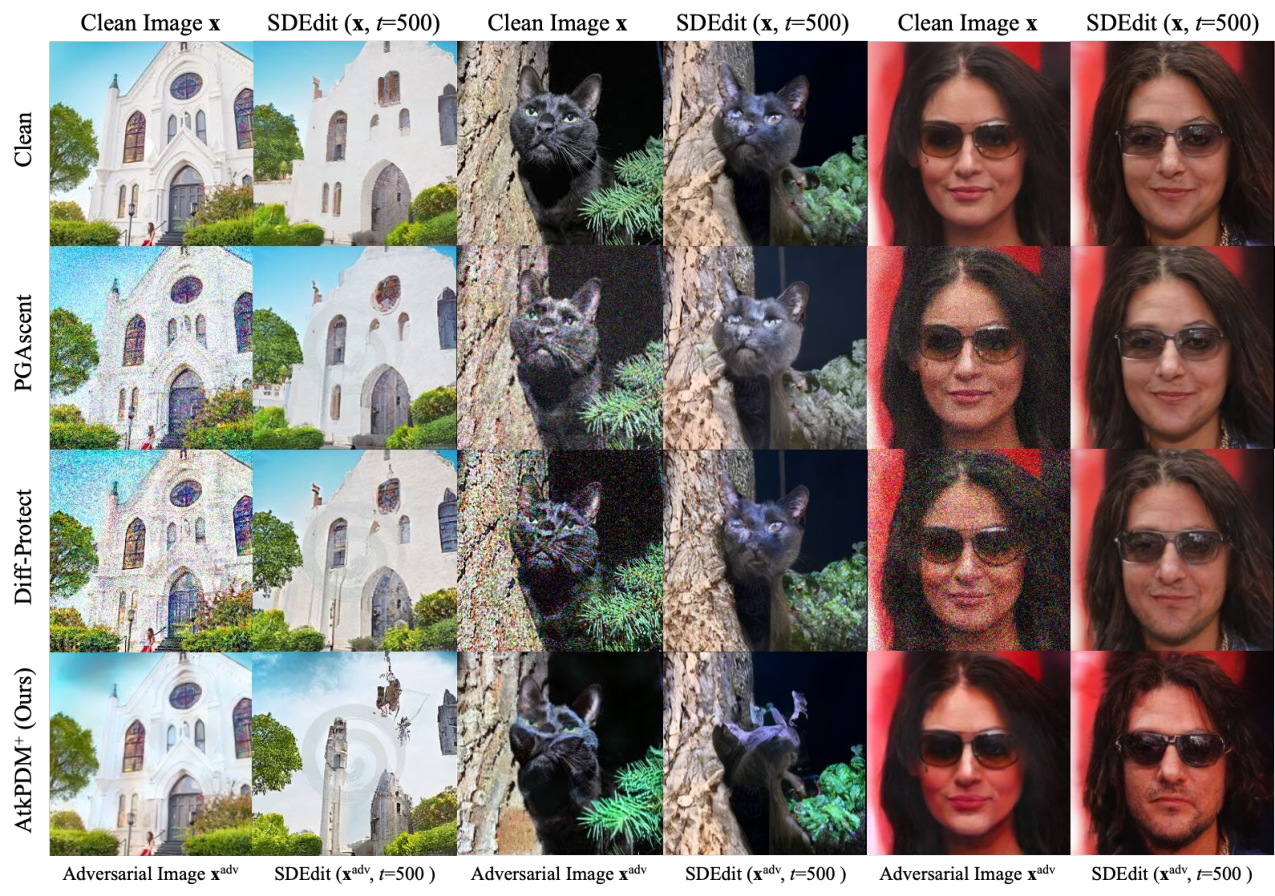
\includegraphics[width=0.79\linewidth]{figures/qualitative_results.pdf}
\caption{Qualitative results compared to previous methods: our adversarial images can effectively corrupt the edited results without significant fidelity decrease. The same column shares the same random seed for fair comparison.
}
\label{qualitative}
\end{figure*}

\begin{table*}
    \centering
    \small{
    \begin{tabular}{lc|ccc|cccc}
        \toprule
        \multirow{2}{*}{Losses} & \multirow{2}{*}{VAE} & \multicolumn{3}{c|}{Adversarial Image Quality} & \multicolumn{4}{c}{Attacking Effectiveness} \\ 
         & & SSIM $\uparrow$ & PSNR $\uparrow$ & LPIPS $\downarrow$ & SSIM $\downarrow$ & PSNR $\downarrow$ & LPIPS $\uparrow$ & IA-Score $\downarrow$ \\
        \midrule
        $\mathcal{L}_\text{semantic}$ &  & 0.37 $\pm$ 0.09  & 28.17 $\pm$ 0.22 & 0.73 $\pm$ 0.16  & 0.89 $\pm$ 0.05 & 31.06 $\pm$ 1.94 & 0.17 $\pm$ 0.09 & 0.93 $\pm$ 0.04 \\
        $\mathcal{L}_\text{semantic}$ & \checkmark & 0.80 $\pm$ 0.05 & \second{29.78} $\pm$ 0.42 & \second{0.17} $\pm$ 0.03 & 0.82 $\pm$ 0.05 & 30.43 $\pm$ 0.75 & 0.15 $\pm$ 0.06 & 0.92 $\pm$ 0.04 \\
        % $\mathcal{L}_\text{semantic}$ + $\mathcal{L}_\text{fidelity}$ &  & 0.12  & 27.90 & 1.08 & \first{0.58} & \first{28.01} & \first{0.93} & \first{0.61} \\ 
        $\mathcal{L}_\text{semantic}$ + $\mathcal{L}_\text{fidelity}$ & \checkmark & \first{0.82} $\pm$ 0.05 & \first{30.30} $\pm$ 0.81 & \first{0.13} $\pm$ 0.03 & 0.90 $\pm$ 0.03 & 31.24 $\pm$ 1.19 & 0.08 $\pm$ 0.03 & 0.96 $\pm$ 0.02 \\
        \midrule
        $\mathcal{L}_\text{attack}$ + $\mathcal{L}_\text{fidelity}$ (Ours) & & 0.75 $\pm$ 0.03 & 28.22 $\pm$ 0.10  & 0.26 $\pm$ 0.04 & \first{0.75} $\pm$ 0.04 & \first{29.61} $\pm$ 0.23 & \first{0.40} $\pm$ 0.05 & \first{0.76} $\pm$ 0.06 \\
        $\mathcal{L}_\text{attack}$ + $\mathcal{L}_\text{fidelity}$ (Ours) & \checkmark & \second{0.81} $\pm$ 0.03 & 28.64 $\pm$ 0.19 & \first{0.13} $\pm$ 0.02 & \second{0.79} $\pm$ 0.04 & \second{30.05} $\pm$ 0.47 & \second{0.33} $\pm$ 0.07 & \second{0.81} $\pm$ 0.06 \\
        \bottomrule
    \end{tabular}
    }
    \caption{Quantitative results of ablation study. The best is in bold and the second best is underlined. Errors denote one standard deviation of all images in our test datasets.}
    \label{tab:loss_ablation}
    \vspace*{-10pt}
\end{table*}



\subsection{Against Defense Methods}
We examine the robustness of our approach against two widely recognized and effective defense methods for defending against adversarial attacks as reported in Table~\ref{tab:defense}.

\subsubsection{Crop and Resize.}
Noted by Diff-Protect, crop and resize is simple yet the most effective defense method against their attacks on LDMs. We also test our method against this defense using their settings, i.e., cropping 20\% of the adversarial image and then resizing it to its original dimensions.


\subsubsection{JPEG Compression.}
Sandoval-Segura et al.~\cite{sandoval2023jpeg} demonstrated that JPEG compression is a simple yet effective adversarial defense method. In our experiments, we implement the JPEG compression at a quality setting of 25\%. The quantitative results in Table~\ref{tab:defense} demonstrate that our method is robust against these two defense methods, with four of the metrics listed in Table~\ref{tab:defense} are not worse than no defenses. Surprisingly, these defense methods even make the adversarial image more effective than cases without defense.


\subsection{Black Box Transferability}
We craft adversarial images with the proxy model, ``google/ddpm-ema-church-256'', in white-box settings and test their transferability to another ``google/ddpm-bedroom-256'' model for black-box attacks. Under identical validation settings, Table~\ref{tab:blackBox} reveals only a slight decrease in attack effectiveness metrics, indicating successful black-box transferability.



\subsection{Effectiveness of Latent Optimization via VAE}
We first incorporate our VAE latent optimization strategy in the previous semantic-loss-based PGAscent. From Table~\ref{tab:loss_ablation}, without using $\mathcal{L}_\text{fidelity}$, latent optimization has significantly enhanced the adversarial image quality and even slightly improved the attacking effectiveness. Adopting latent optimization in our approach enhances visual quality with a negligible decrease in attacking effectiveness. Surprisingly, incorporating our $\mathcal{L}_\text{fidelity}$ with current PGD-based method will drastically decrease the adversarial image quality despite its attack performing better than ours. This may be due to different constrained optimization problem settings.
